\chapter{Operating Cost}\label{ch-doc}
民机设计除了要满足航空公司对飞机安全性及性能的要求,对乘客具有吸引力外,还必须能够为航空公司带来经济效益。通过增加飞机的销售数量,飞机制造商可以收回投入的项目开发成本,并通过进一步的利润积累为新技术的研究和下一代飞机的研发提供资金。因此成功的机型除了技术上的先进性以外,还需要具有良好的经济性,包括较低的购买成本和使用成本等。

民机的经济性分析是总体设计的重要内容,对整个项目的市场成功具有至关重要的作用。飞机项目,尤其是全新的飞机项目的研发时间往往很长,其累计现金流在设计初期直到设计定型,将产品推向市场并获得初始订单之前,一直都为负值。在销售的飞机达到一定数目时才可以收回研发及生产成本,亦即达到盈亏平衡点。由于其所需的巨额的现金投入,使飞机项目的风险巨大。在飞机设计的各个阶段,要对设计方案的经济性和市场前景进行尽可能准确的分析和预测,以增加项目成功的几率。这一任务在设计的初期尤其重要,这一阶段作出的设计决策对飞机的购买成本及使用成本的影响巨大。

\section{成本概念与评估方法}\label{c13.1}
%航空公司对飞机的经济性的评估通常会考虑下面几个方面的成本
%\begin{itemize}
%\item[-]资本成本-购买飞机的成本,亦即飞机的价格
%\item[-]直接使用成本-使用飞机进行商业运营的成本
%\item[-]间接使用成本-维持航空公司运营的成本
%\item[-]总使用成本-提供商业航空服务的所有成本
%\item[-]每座公里成本-平均到每座位公里的成本
%\end{itemize}

\subsection{全寿命使用成本}\label{c13.1.1}
航空公司使用一架飞机完成特定航线任务涉及三个方面的成本,飞机的购买成本、使用成本和支撑飞机使用的成本,如维修和备件成本等。而一架飞机从下线和投入航线运营,到最后退役所经历的时间长达$20\sim30$年。

全寿命周期成本应该包括与飞机直接相关的成本和支撑飞机运行的非直接成本。非直接成本的计算与航空公司的运行方式和财务计算方法有直接的关系,不同航空公司的计算方法得出的结果差异比较大。

%Curren等提出了将基于一般性规则与偶然性因素(Genetic-Casual)相结合的方法用于%
%制造成本和全寿命周期成本的估算研究中~\cite{curren05}。Scholz
%提出了与常规DOC方法略有区别的DOC$_{\textrm{sys}}$方法~\cite{scholz},%
%与传统DOC计算的主要区别是加入了针对飞机系统进行评估的有关方法,将能够区别不同飞机的%
%成本都记入DOC$_{\textrm{sys}}$,例如在对比两人机组飞机时,可以将机组成本忽略,%
%而将原本分类为IOC的维持备用件库存所发生的成本记入直接使用成本。

民机的总使用成本(TOC)主要由以下几个元素构成,包括与飞机有关的使用成本(Airplane Related Operating Cost AROC),或称直接使用成本(DOC);与乘客服务有关的使用成本;与货运服务有关的使用成本;与飞机地面系统有关的使用成本等,其中后面三个方面的内容也统称为间接使用成本(IOC),非直接成本在总的使用成本中大约占$15\%\sim50\%$,在缺乏可靠数据估算的情况下,可以假定IOC的数值近似等同于为DOC,而将重点放在DOC的计算上。DOC中又包括两个方面的内容:所有权成本或资本成本,和现金使用成本(CAROC)。具体的划分如图\ref{fig_toc}所示。
\begin{figure}
\begin{center}
  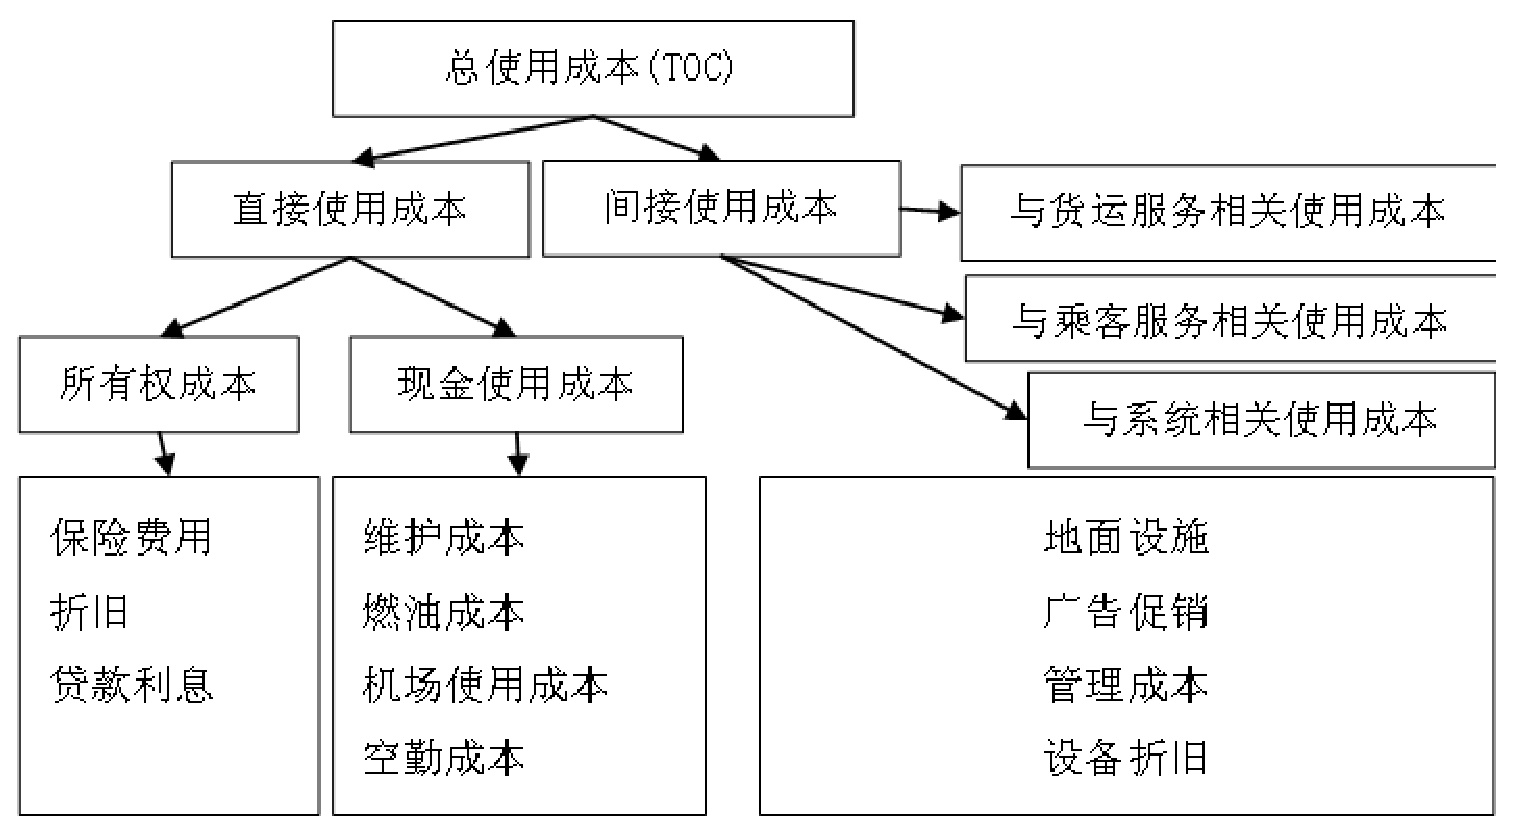
\includegraphics[width=0.8\textwidth]{doc/toc_composition.eps}
  \caption{飞机总的使用经济性(TOC)的构成}
  \label{fig_toc}
\end{center}
\end{figure}

飞机的经济性可以使用下述不同的指标进行衡量,反映飞机直接使用成本的指
标有:
\begin{itemize}
\item[(1)]飞行小时成本(DOC美元/飞行小时)
\item[(2)]航段成本(DOC美元/航段)
\item[(3)]座海里成本(DOC美元/座海里)
\item[(4)]吨海里成本(DOC美元/吨海里)
\end{itemize}
反映飞机制造成本的指标包括:
\begin{itemize}
\item[(1)]单位空机成本(美元/$W_{oe}$)
\item[(2)]单位商载成本(美元/$W_{pl}$)
\end{itemize}

式中,$W_{oe}$和$W_{pl}$分别为使用空机重量(吨)和最大使用商载重量(吨)。其中,最常用的是民机经济性评价指标是座海里成本。

\subsection{经济性评估方法}\label{c13.1.2}
经济性评估可以使用不同的经济性指标进行。准确估算飞机的经济性是一项非常困难的工作,却又是概念设计和初步设计阶段一项非常重要的工作。在这一阶段有关设计方案的数据非常缺乏,众多参数都有待确定。这又为准确估算飞机成本带来了很大的困难。

飞机成本估算的常用方法包括自下而上的方法,从估算零件的成本到整个产品的成本,其中涉及对大量数据的处理,而估算的结果受到多种因素的影响,在概念设计阶段,当许多细节尚未确定时,很难采用这种方法。

第二种方法是基于历史数据进行类比分析来进行估算,这种方法对新飞机研发成本的估算存在很大困难,尤其是当飞机间的技术水平差距较大时,需要采用合适的修正因子。可以利用的方法包括案例推理(Case-Based Reasoning, CBR)以及使用神经网络和模糊逻辑的工具等。

第三种方法通过建立成本与关键设计参数间的关联关系来进行,因而称为“参数法”(Parametric Costing)。将DOC和设计参数进行关联得到的成本模型与重量、性能、几何等模块相集成,进行各种设计参数对经济性影响的灵敏度研究,是目前越来越多采用的方法。

其他在财务分析领域使用的方法包括作业成本法(Activity-Based Costing,ABC)和薄利成本法(Lean Costing),这些方法代表了另一类将成本与资源使用和工程活动进行映射的方法。随着计算建模技术,特别是CAD技术的发展,初步设计阶段可以使用越来越多的详细数据,这一发展趋势使得对部件的制造成本信息的把握越来越准确,尤其是对传统金属类结构形式。多种成本估算方法相结合,能够为初始设计阶段的有效决策提供更多的依据。

\section{飞机经济性分析与计算方法}\label{c13.2}
飞机的经济性,与安全性、舒适性和可靠性一起,是民用客机设计的重要指标。民航市场的激烈竞争,决定了民机经济性的优劣往往对民机项目的成败起着关键的作用。在概念设计和初步设计阶段,需要对竞争机型和不同设计方案的经济性进行分析,尤其是直接使用成本,以便选择合适的参数来达到设计方案的综合最优,提高在市场上取得成功的几率。

市场成功是民机设计经济性指标优劣的重要反映。在考虑经济性的设计过程中,首先应基于对预期目标市场和对航空技术发展水平的分析,对不同方案的成本进行估算,作出对技术选择和方案参数选择的评估,最终完成飞机设计参数的确定。

设计方案对经济性的影响主要体现在以下几个方面,飞机的气动外形参数、结构设计和材料选择将影响飞机的起飞重量和结构可靠性,进而影响到飞机的使用成本。金属结构的飞机设计已经相对成熟,但其能够带来的性能改进也变得有限;提高设计的可靠性,减少维护时间是提高经济性的另一个有效手段,现有维护时间和维护材料成本的估算方法大多是基于金属结构的数据,因此可以应用于目前的估算工作中。燃油成本在飞机的使用成本中占有显著的比重,因此发动机性能,尤其是发动机的燃油效率将直接影响飞机的使用成本;此外,影响飞机使用成本的另一个因素是飞机的全机气动效率。

虽然存在不少经济性分析的模型和工具,但大部分方法和公式都来源于国外的数据和经验公式,不一定完全满足国内的现状,因此需要进行数据和模型的不断修正。采用这些模型和公式计算得出的结果尽管不一定完全准确,但可以用于方案设计阶段进行不同方案经济性的对比。随着方案的进一步细化和数据的不断积累,估算的精确度也会不断提高。

现代民机设计一般采用先进发动机技术,达到增大推力、减少油耗、降低噪声和排放的目的,油耗降低带来燃油成本的降低,可靠性和维修性的改善会降低维修成本。但新技术的研发又提高了发动机的自身成本。在新一代民机中,复合材料的使用超过$50\%$,复合材料具有显著的重量优势,以及良好的可靠性和损伤容限特性,从
而改善了维修间隔时间,降低了维修成本;但由于其制造成本较高而提高了使用成本。此外,电传操纵系统在现代民机中广泛使用,由于需要采用余度技术以确保其可靠性,增加了制造成本。但其对设计的影响,如可以采用放宽静稳定性、载荷抑制、阵风抑制、颤振抑制等功能,又减轻了飞机重量,飞机气动效率的提高减少了燃
油成本。从以上举例可以看出,所有新技术的采用都存在一方面提高研发制造成本,另一方面又降低使用成本的因素。因此需要对可能影响新技术的因素进行综合分析,才能得出最终对经济性的影响结果,从而作出是否使用特定的新技术以及使用的深浅程度的决定。

\subsection{直接使用成本(DOC)}
直接使用成本的计算是一项关键的工作,也是一件困难的工作。从航空工业的发展初期,就将成本的预估和控制作为各个设计阶段的重要内容。早在1944年美国航空运输协会(Air Transport Association of America,ATA)就发表了第一个被广泛接受的直接使用成本的估算方法,之后经过多次改进,并逐步从最早的活塞式发动机扩展到了采用涡轮发动机的飞机上。目前广泛使用的方法就是基于1976年的ATA方法。此外,欧洲也发展了自己的经济性的评估方法,通常称为AEA方法。

各种DOC的估算方法对成本项目的划分基本上是一致的,DOC计算中涉及的成本项目主要包括以下内容:资本成本、机场使用成本、燃油成本、维护成本,以及空勤成本等。各项具体成本项中所包含的具体内容如表\ref{table_docsum}所示。

\begin{table}
\centering \caption{飞机直接使用成本(DOC)的计算元素}
\label{table_docsum}     % Give a unique label
%\begin{tabular}{lp{3.8cm}lp{6cm}}
\begin{tabular}{p{0.20\textwidth}p{0.68\textwidth}}
\hline \hline
资本成本&贷款额度,利率,期限,残值,保险率,寿命期限,配件投资成本等 \\
机场成本&导航服务,降落费用,地面服务,旅客服务,民航基础设施建设基金收费等 \\
机组费用&平均薪资水平,包括飞行员,空乘\\
燃油成本&轮档时间,轮档燃油 \\
维护成本&发动机维护成本,飞机维护成本 \\
\hline \hline
\end{tabular}
\end{table}

民机直接使用成本的计算与飞行任务剖面和飞机的性能直接有关,其中涉及的性能参数包括轮档时间、轮档燃油等。依据飞机设计手册,通常选取的飞行任务剖面如图\ref{fig_flight_profile}所示,其中包含两个部分,第一部分为正常的飞行任务剖面,第二部分为备份燃油航段。其中备用油的规则由以下三个部分组成,包括5\%任务用油,200海里备降转飞用油,和1500英尺高度30分钟待机用油。飞行任务剖面中各航段的燃油计算规则如表\ref{table_fortoc}所示。其中给出的燃油比系数为初步的估计值,或为采用性能计算模块获得的更为准确的数据。

\begin{table}
\centering \caption{DOC计算中轮档燃油的简化计算数据}
\label{table_fortoc}     % Give a unique label
%\begin{tabular}{lp{3.8cm}lp{6cm}}
\begin{tabular}{p{0.08\textwidth}p{0.32\textwidth}p{0.22\textwidth}p{0.18\textwidth}}
\hline \hline 航段 & 描述 & 燃油比($\frac{w_{i+1}}{w_i}$)& 时间(分钟) \\
\hline 1&发动机启动、预热与滑行 &0.98 &7 \\
2&起飞,初始爬升至1500英尺 &0.98 & 计算得出 \\
3&加速,爬升到巡航高度 &0.98 & 计算得出\\
4&巡航 &计算得出&计算得出 \\
5&下降 &0.99 & 计算得出 \\
6&进场与着陆 &0.992& 6\\
7&滑行  &0.99 &7 \\
\hline
8&过失进场 &0.98 & 计算得出\\
9&爬升至20000英尺 &0.98 & 计算得出  \\
10& 20000英尺巡航到备降机场 &计算得出&计算得出 \\
11&下降至1500英尺 &0.99 &计算得出 \\
12&进场与着陆 &0.992& 6\\
\hline \hline
\end{tabular}
\end{table}

\nomenclature{$W_E$}{飞机的运营空重}
在DOC的构成中,各项成本所占的比重都不同,其中最主要的三个构成元素分别为资本成本、燃油成本和维护成本。由于在飞机的采购或租赁中可以采用的财务规则的差异,资本成本的计算存在很多方法,但都与飞机的总投资有关,总投资包括在飞机和发动机上的投资,还包括在配件和地面辅助设备上的投资。在配件和地面辅助设备上的投资通常按照飞机或发动机总价的百分比来确定。在方案设计阶段对飞机机体价格的估算主要是通过关联飞机结构重量和飞机目录价格(list price)近似得到,根据波音的数据可以得到飞机机体的单价估算公式为:
\begin{equation}
\label{eq_boeingprice} P_{tc}=0.0010W_{e}^{0.96}
(\mbox{百万美元},2007\mbox{年})
\end{equation}
式中,$W_e$为飞机的运营空重(单位是lb),图\ref{fig_airplane_price}给出了飞机%
价格与运营空重的经验关系。



\begin{figure}
\begin{center}
  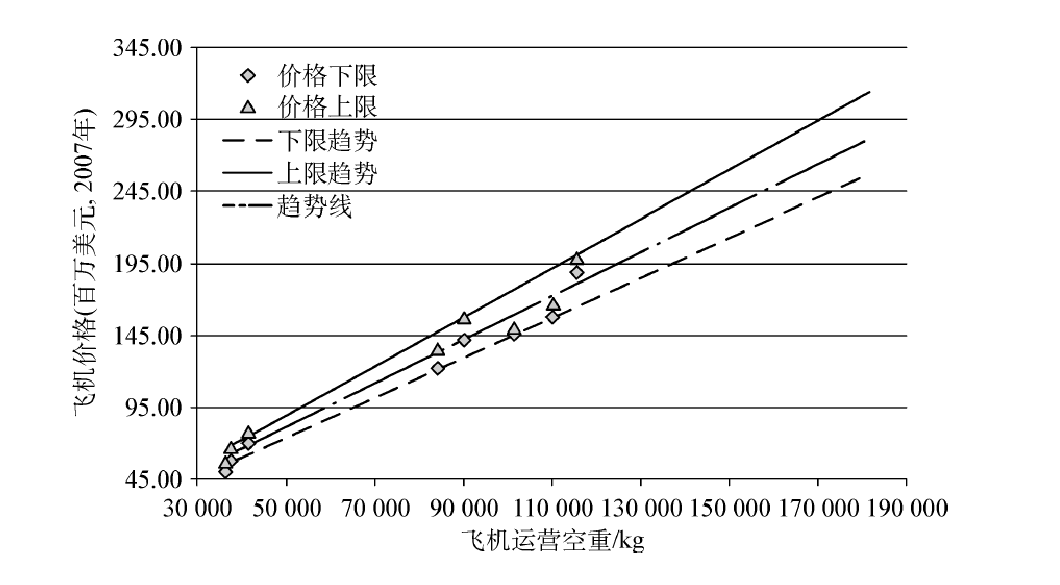
\includegraphics[width=0.8\textwidth]{doc/price_new.eps}
  \caption{飞机机体价格与运营空重间的经验关系}
  \label{fig_airplane_price}
\end{center}
\end{figure}

发动机的价格可以通过关联发动机的推力和燃油效率SFC来得到估算公式为:
\begin{equation}
\label{eq_engineprice}
P_e=1.36×1.5561×[0.3857×(\frac{T_{c}^{0.88}}{SFC^2.58})+0.7286]
(\mbox{百万美元},2007\mbox{年})
\end{equation}
式中,$T_{c}$为发动机的巡航推力(单位为千lbf)。SFC为发动机的燃油效率[单位为lb/(h·lbf)],式中的系数是将货币修正到2007年美元的系数。
\nomenclature{$T_{c}$}{发动机的巡航推力}


飞机的资本成本与资金的来源和使用方式有很大的差别,通常航空公司需要进行详细的评估。一般来说,航空公司可以采用购买和租赁的形式取得飞机的使用权。在这两种形式下,资本成本的计算是不同的,同时还受到各种不同财务制度的影响。

在贷款购买模式下,资本成本的计算是基于飞机机体和发动机的总价来得到的,包括贷款成本、折旧成本和保险成本三个部分。贷款成本的计算可以按如下方式进行,假设贷款总额为$A$,总的还贷次数为$n$,每期还贷利率为$\beta$,每期还款额为$a$,还款年限为$m$,采用等额还本付息方式,每期还款额由以下公式计算
\begin{equation}
a=\frac{A\beta}{1-\frac{1}{(1+\beta)n}}
\label{eq_captitalcost_buy}
\end{equation}
年度利息为
\begin{equation}
i=\frac{n·a-A}{m} \label{eq_captitalcost_interests}
\end{equation}

折旧成本的计算针对飞机机体和发动机的总价格,考虑折旧后的残值和折旧年限用
公式\ref{eq_deprecalc}进行计算。
\begin{equation}
C_d=(P_a+P_e)\frac{1-r}{d_m}
\label{eq_deprecalc}
\end{equation}
式中,$r$是残值所占的百分比,$d_m$为折旧年限。

如果已知飞机和发动机总价,以及保险费率,年度的保险成本计算可以由式%
\ref{eq_doc_insurance}得出
\begin{equation}
\label{eq_doc_insurance} P_{ins}=P_t·r
\end{equation}

机场服务的成本计算将机场服务的成本分解为导航服务费、进近指挥费、航空业务服务费,以及机场地面服务费,与机场服务密切相关的旅客餐食项目也列在此处。导航服务费通常按飞行的里程来计算,进近指挥费根据飞机的降落重量来计算,旅客餐食是根据座舱等级,依据旅客数目进行计算。航空业务服务费和机场地面服务费的计算较为复杂,两者的计算与飞机的设计特点存在一定的联系。

空勤成本在DOC中的计算一般取决于轮档时间,飞机的起飞重量(飞机的种类)和平均单位时间的薪金水平。空乘人员的薪金水平和计算方法因航空公司不同而变化较大,计算中所采用的空乘人员的月薪金水平可以根据我国的平均水平来计算。

燃油成本取决于飞机完成特定航线所消耗的轮档燃油和燃油单价,其中轮档燃油的计算根据典型的任务剖面来进行。计算结果与飞机的性能参数,如巡航速度、巡航时的升阻比,以及发动机的油耗性能之间存在密切的关系。燃油成本在DOC中的比重随着燃油价格的增加而增加,是航空公司运营成本中的重要元素,也反映出改善发动机的油耗特性对改善DOC性能有很大的意义。

维护成本的计算通常分解为飞机维护成本和发动机维护成本,飞机维护成本的计算包括人工成本和材料成本,取决于飞机每年平均的飞行小时、单次任务的飞行时间和飞机的结构重量,在还没有飞机的结构重量估算时,可以采用飞机的运营空重。

在计算DOC的过程中,各种政策性收费,例如我国征收的民航基础设施建设基金也应考虑在内。政策性收费有时是针对特定机型的,比如针对排放严重的老机型等。

\subsection{非直接使用成本(IOC)}
概括来讲,非直接使用成本就是与飞机具体的设计特征没有直接关联的成本项目。这些项目是航空公司开展商业运营活动所必不可少的支出,主要包括下面的一些内容:
\begin{itemize}
\item[(1)]地面设施的所有或租赁,以及使用成本,包括办公室,值机柜台等。
\item[(2)]地面设备成本,包括设备维护,折旧等。
\item[(3)]管理及维护费用。
\item[(4)]总部办公成本。
\item[(5)]广告,销售,以及公关成本。
\item[(6)]票务服务成本,包括订票服务。
\item[(7)]培训成本。
\item[(8)]客户服务成本。
\end{itemize}
非直接成本的计算因航空公司不同而差别很大,作为一个粗略的近似,基于B747%
(四发),DC-10(三发)和两发飞机的统计数据,可以采用如下的公式近似计算%
间接使用成本。
\begin{equation}
IOC=R^{-0.41}[1.19\times{10^{-4}W_{to}}+(0.11+1.17f_1)N_p-3.69](\mbox{百万美元},2007\mbox{年})
\end{equation}
式中,$R$为飞机的任务航程,$W_{to}$为飞机的起飞重量,$f_1$为上座率(乘客数与总座位数之比),$N_p$为总的座位数。从中可以看出,间接使用成本和上座率及飞机的最大起飞重量有关。
\nomenclature{$f_1$}{上座率}

一般来说,设计师对间接使用成本的影响能力是有限的,在设计中需要考虑的主要内容包括地面设备的通用性,以减少购置或租赁新设备的成本,另外,增加驾驶舱设计的共性也有助于降低飞行员的培训成本。

\section{DOC算例}\label{c13.4}
本节以一个具体的民用飞机设计为实例,计算该设计方案的直接使用成本。作为计算实例的是150座级中短程客机,与空客A320和波音B737属于同一个级别,飞机的基本设计参数如表\ref{table_docexample}所示。

\begin{table}
\centering \caption{150座级飞机的基本参数}
\label{table_docexample}     % Give a unique label
%\begin{tabular}{lp{3.8cm}lp{6cm}}
\begin{tabular}{p{0.28\textwidth}p{0.16\textwidth}||p{0.20\textwidth}p{0.16\textwidth}}
\hline \hline 设计参数 & 数值 & 设计参数 & 数值 \\
\hline 最大起飞重量 &73500 kg &发动机型号 &CFM56-5B \\
飞机运营空重 &42175 kg   &发动机台数  &2 \\
载客数  &150 &巡航SFC &0.63 1/hr\\
驾驶员数  &2  &函道比 &5.3 \\
机组人数  &3  &巡航推力   &28.7 kN\\
最大巡航速度   &487 kn  &经济巡航速度  &454 kn\\
\hline \hline
\end{tabular}
\end{table}

在DOC的计算中,假设航段里程为1000 n mile(1852 km),年飞行时间为3000h,计算所用的轮档时间为157min,轮档燃油为6241 kg,由此得出年利用率为1146架次。
根据飞机与发动机的基本参数,人民币汇率采用6.83,可以近似估算出飞机机体和单发发动机的价格如下:

飞机机体价格=$0.00101\times(42175\times2.20462)^{0.96}\times6.83=405.88$百万元

发动机单发价格=$0.5\times1.36\times1.5561\times[0.3857\times(T^{0.88}/SFC^{2.58})+0.7286]=52.65$百万元

飞机的总价为机体价格与两台发动机价格的总和511.18百万元。考虑到飞机配件、发动机配件和地面支持设备的投资额度分别占飞机机体价格、发动机价格和飞机总体价格的百分比分别为8%,20%和1.7%,可以计算得出总投资额为573.40百万元。

如果采用租赁形式,假设租赁保证金比例为10%,租赁期12年,租金为每月支付,年贴现率6%,承租期满的飞机残值为30%,租赁手续费为租金的5%,则每航段租金可以计算为:45333元

假设机长飞行员月薪15000元,副机长飞行员月薪10000元,空乘月薪9000元,其他间接成本占月薪的20%,则计算得出每航段空勤成本为:2717元

每航段燃油成本的计算为:$5.637\times5000=28185$元

民航基础建设基金为:$4259$元

维修成本包括飞机维修成本和发动机维修成本,分别计算为:4408元和2919元,共计7319元。

旅客餐食成本的计算为:$25\times8+16\times142=2472$元

机场服务成本包括如下各项:
导航费与进近指挥费为$0.2\times1852+5\times73.5=737.9$元;机场航空服务收费由于所在机场不同而有所不同,其包括起降费,停场费,客桥费,旅客服务费和安检费,按平均水平计算可以得出:

起降费:$1162.5+23.25\times(73.5-50)=1708.88$元

停场费:$1708.88\times15\%\times365/1146=81.64$元

客桥费:100元(一小时以内)

旅客服务费:$150\times45.75\times0.7=4803.75$元

安检费:$150\times6.25+2\times39.5=1016.5$元

机场地面服务费包括一般代理费,配载/通信/集装设备/旅客及行李服务收费,货物及邮件服务收费,客梯/装卸/地面运输服务,飞机服务和飞机勤务收费,各项收费的计算分别如下:

一般代理费:50元

配载等服务,货物及邮件服务,以及客梯等服务收费:
$16.22\times(33+28+6)=1086.74$元

飞机服务:$120\times2.3=276$元

飞机勤务:$150+160\times0.5\times1.5=270$%

将以上各项收费汇总,可以得出每航段机场服务收费为:9279.23元。

综合上述DOC中的所有元素,可以得出每航段DOC的计算结果为:96212.83元,每座公里DOC为0.35元,每公里DOC为51.95元,每日直接运营成本为302108元。

\section{基于经济性的设计}\label{c13.4}
建立飞机方案的经济性分析模型的目的是通过经济性的分析对比不同设计方案,结合市场分析,研究不同设计参数的影响。基于经济性的设计是指将经济性指标作为飞机参数综合的迭代过程中的目标函数之一,与性能、可靠性、舒适性和安全性等指标同时考虑。

经济性分析对民机设计尤为敏感,是航空公司进行机型选择的出发点和落脚点,因此需要将经济性作为设计流程的有机组成部分进行优化,构建基于经济性的一体化设计体系,如图\ref{fig_economic_design}所示。%
\begin{figure}
\begin{center}
  
\includegraphics[width=0.8\textwidth]{doc/economic_design.eps}
  \caption{基于经济性的方案设计流程}
  \label{fig_economic_design}
\end{center}
\end{figure}
影响民机经济性指标直接使用成本的主要因素包括飞机的航程,座位数,发动机的油耗等。飞机的性能指标通过轮档时间与轮档燃油影响飞机的直接使用成本,不同设计参数对性能和飞机重量的影响最终反映在飞机的使用成本上面。在建立了飞机的直接使用成本模型以后,可以进行设计参数的灵敏度分析和优化研究。以150座级的飞机设计为例,图\ref{fig_docrange,fig_docseats,fig_docsfc}中分别给出了航程、
座位数和发动机油耗(SFC)对飞机直接使用成本的影响曲线。%
\begin{figure}
\begin{center}
  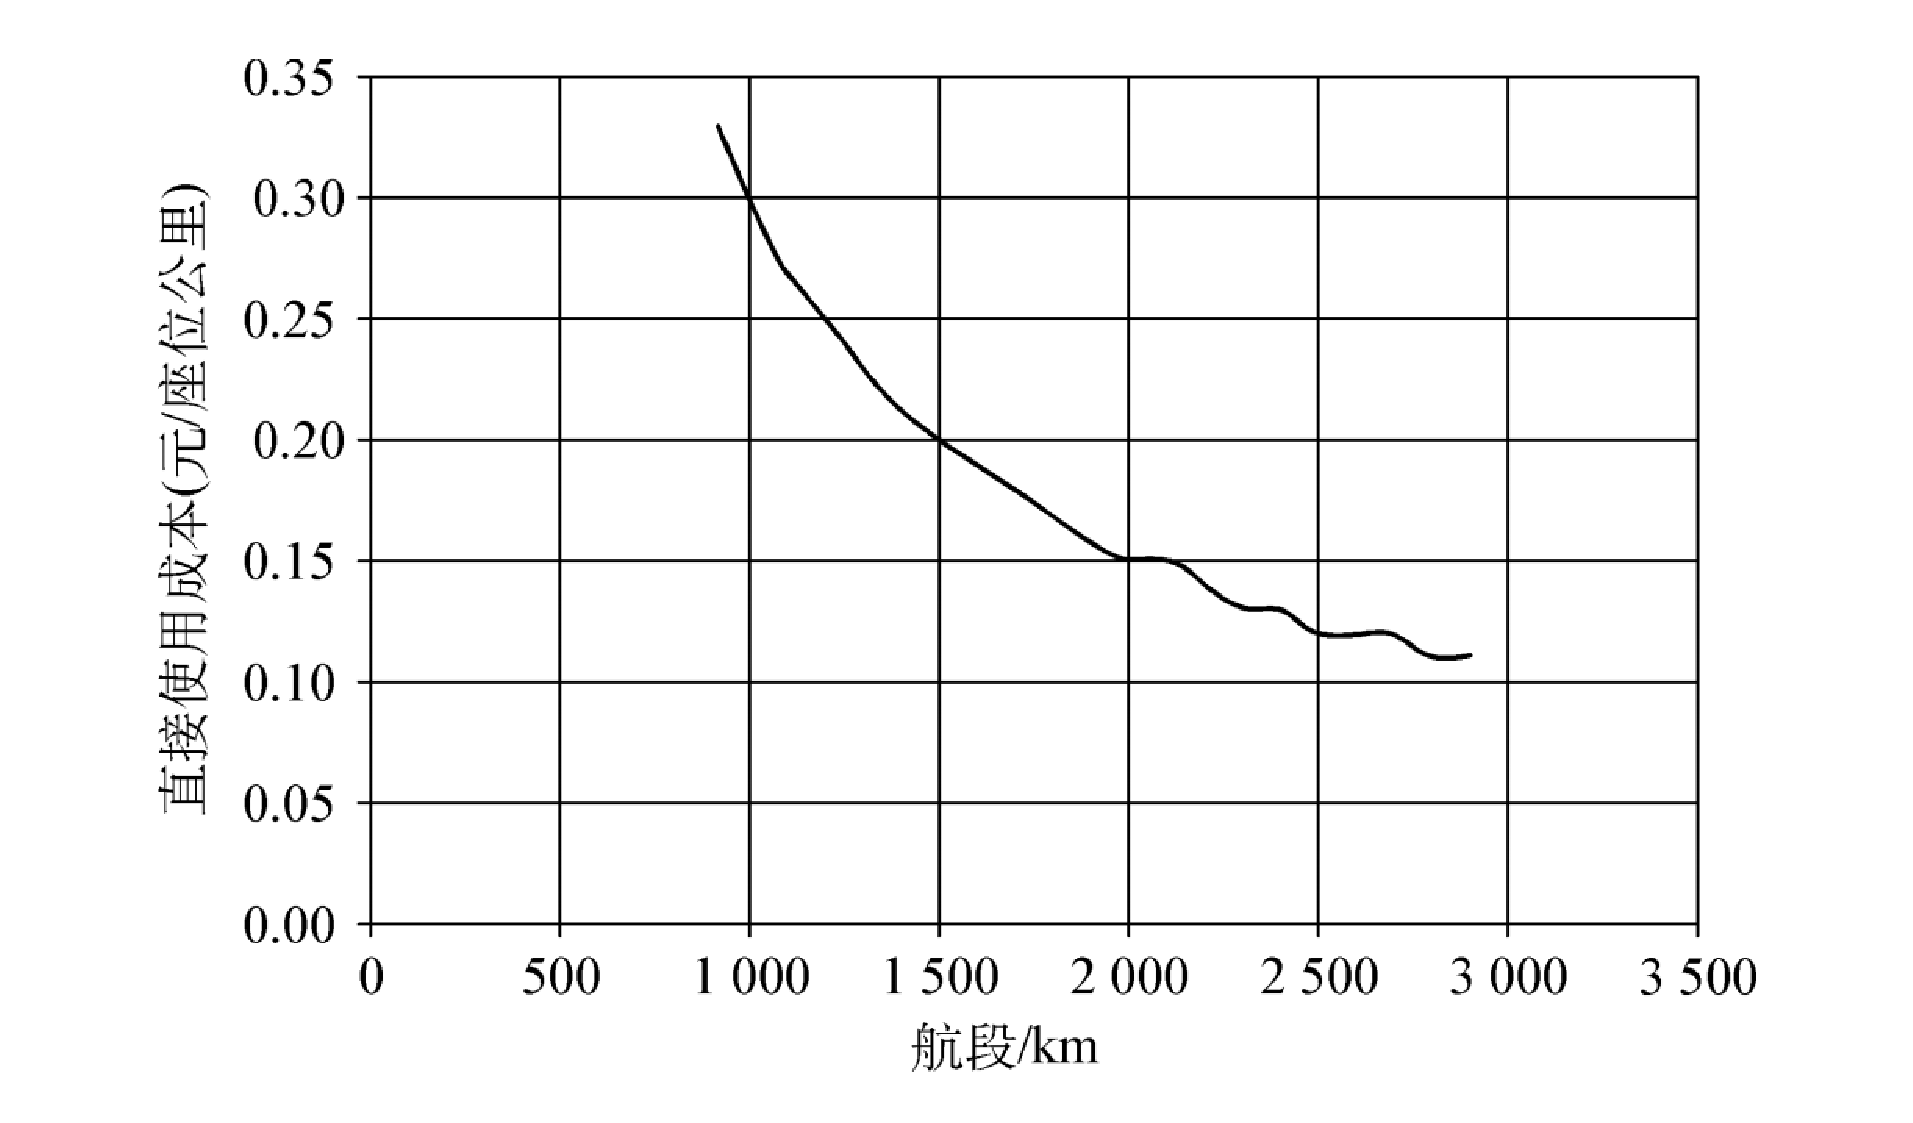
\includegraphics[width=0.8\textwidth]{doc/doc_range.eps}
  \caption{航程对直接使用成本的影响}
  \label{fig_docrange}
\end{center}
\end{figure}
\begin{figure}
\begin{center}
  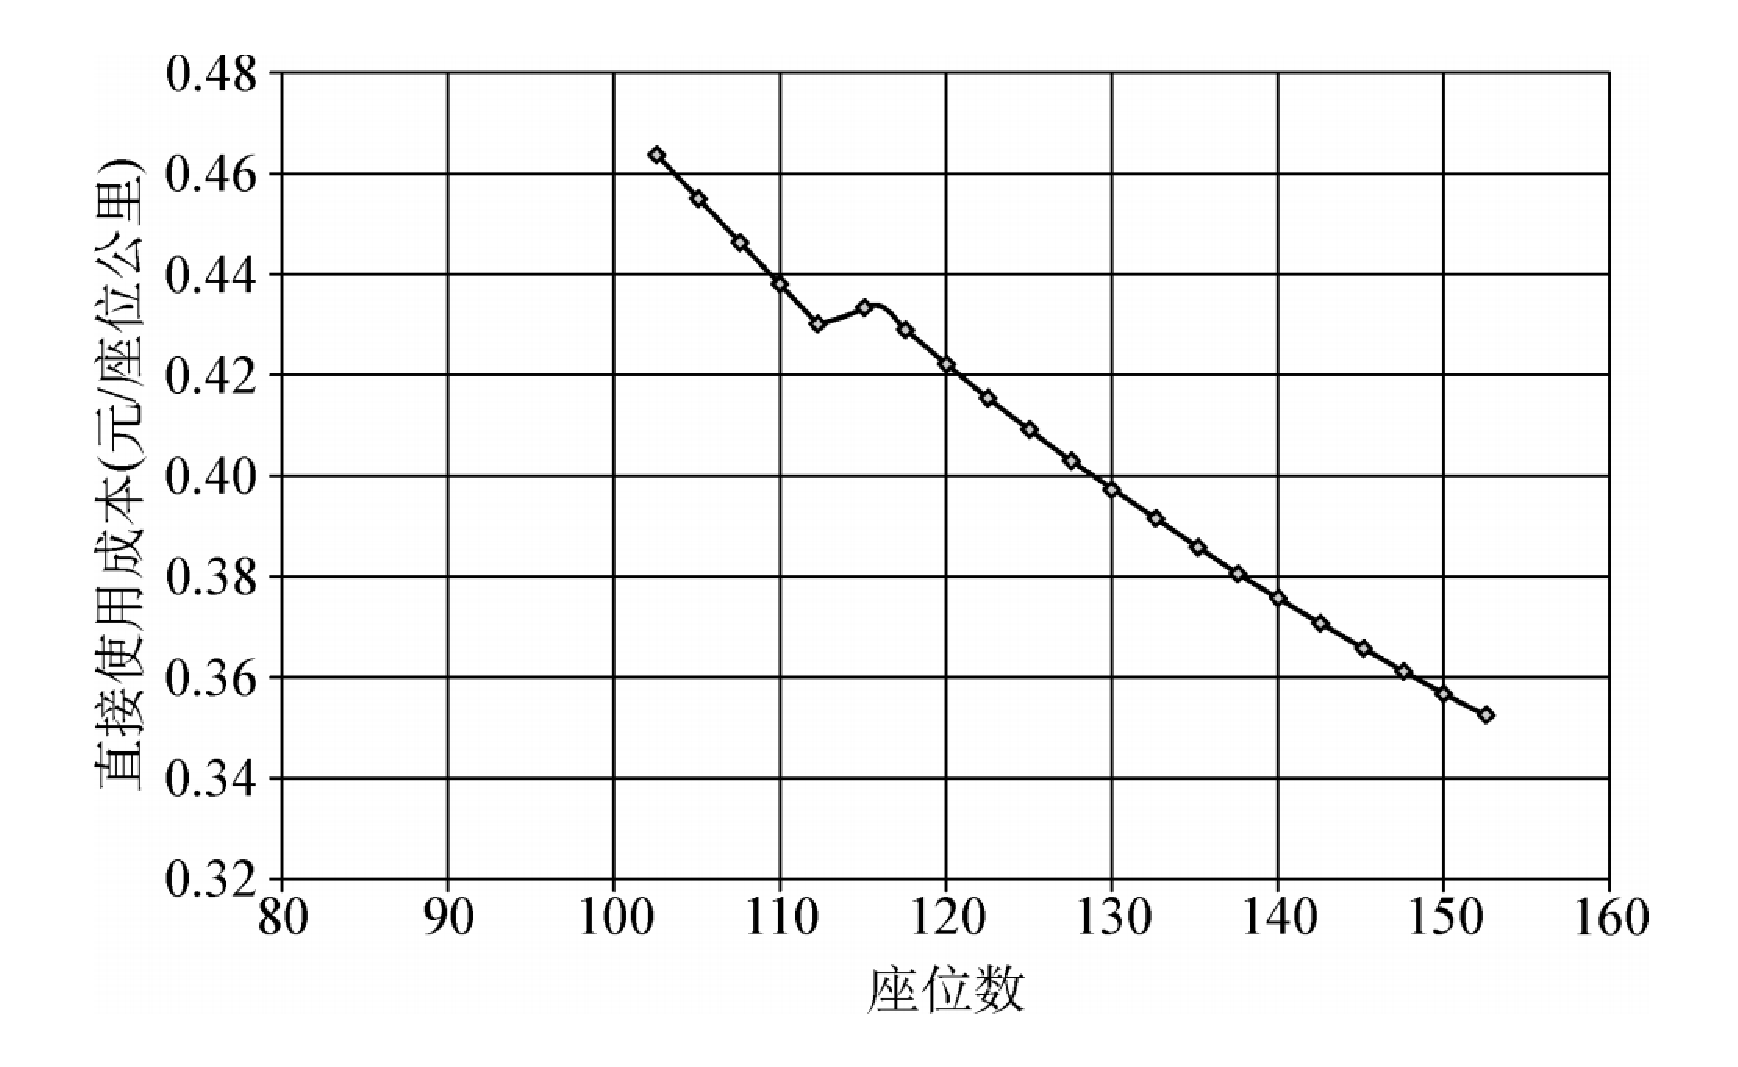
\includegraphics[width=0.8\textwidth]{doc/doc_seats.eps}
  \caption{座位数对直接使用成本的影响}
  \label{fig_docseats}
\end{center}
\end{figure}
\begin{figure}
\begin{center}
  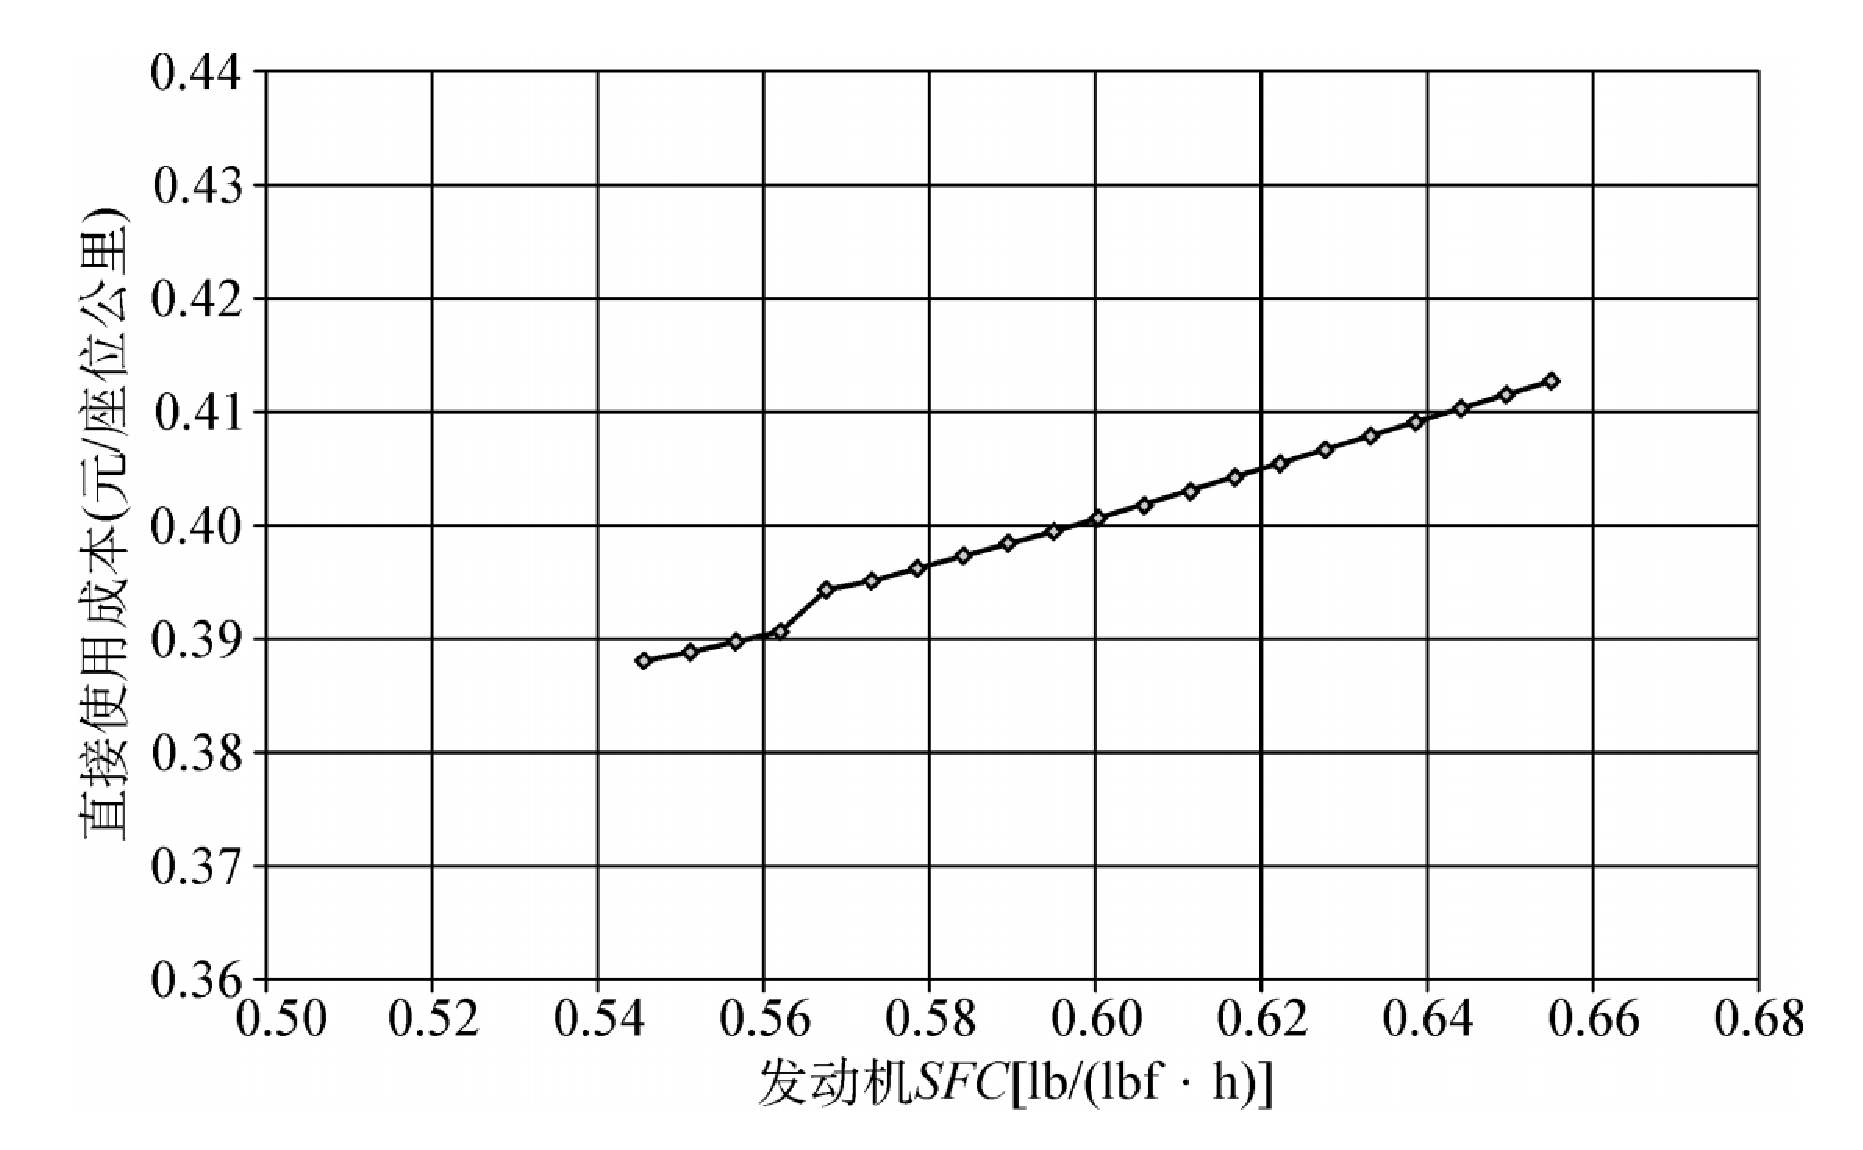
\includegraphics[width=0.8\textwidth]{doc/doc_sfc.eps}
  \caption{发动机油耗SFC对直接使用成本的影响}
  \label{fig_docsfc}
\end{center}
\end{figure}

在有关经济性的设计决策中,应充分考虑所面临的经济环境的不确定性,在设计中利用模糊逻辑等有关的决策工具,以便得出尽可能最优的设计方案。
